\section{Experimental Facility and Methodology} \label{s:experiment}

This section will describe the experimental facility, as it is currently assembled, and the methodology used to test the piston valve.

% talk about basic methodology of experiments and testing, introduce the structure of the section


% section for experimental facility, comparison of rupture disk and piston valve test set ups
\subsection{Experimental Facility} \label{ss:facility}

%
\begin{figure}[tb]
    \vspace{16pt}
    \centering
    \begin{subfigure}[t]{0.6\textwidth}
        \centering
        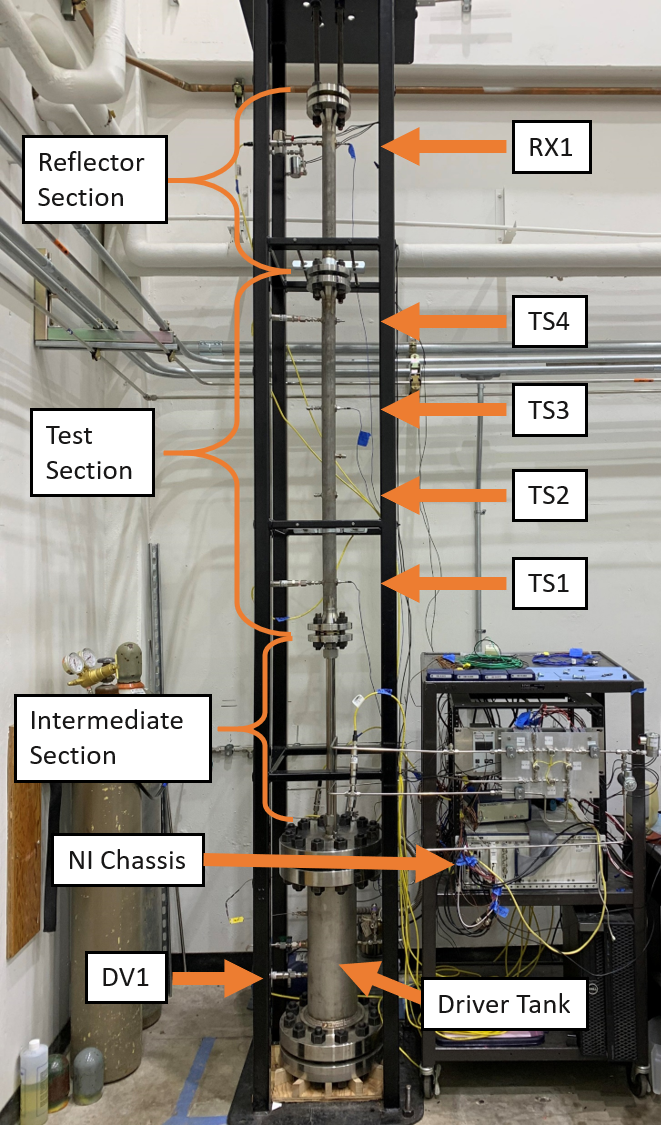
\includegraphics[width=2in]{experiment/photos/HENRI_labels.png}
        \caption{HENRI out-of-pile experimental facility.}
        \label{fig:HENRI Facility}
    \end{subfigure}
    \hfill
    \begin{subfigure}[t]{0.35\textwidth}
        \centering
        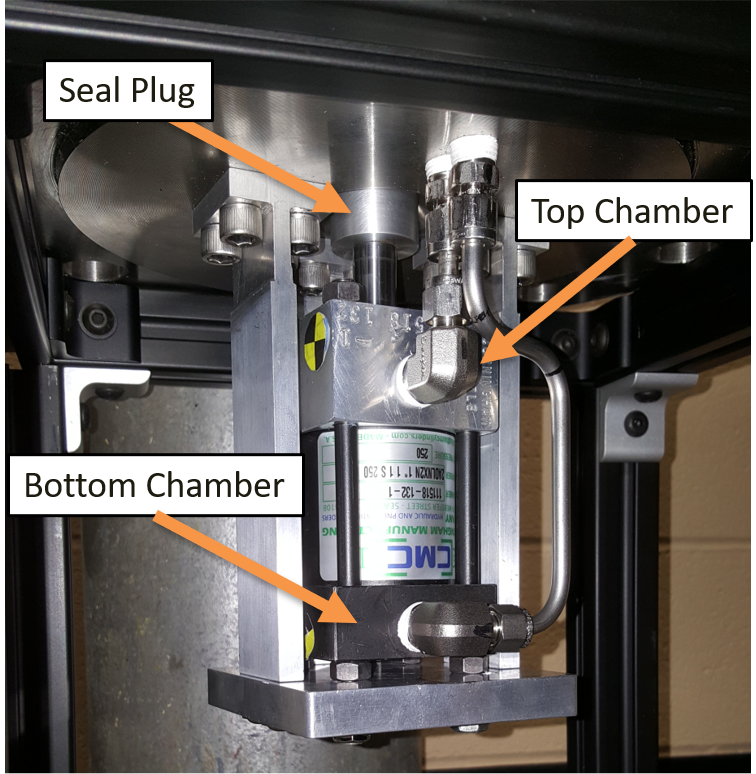
\includegraphics[width=0.9\textwidth]{design/photos/piston_mount_chambers.png}
        \caption{Piston valve attached to driver tank flange with mount, used for seal durability testing.}
        \label{fig:piston valve}
    \end{subfigure}
    \caption{HENRI experimental facility for piston valve testing.}
    \label{fig:facility}
    \vspace{16pt}
\end{figure}
%

% P&ID, photos, etc. of facility -- highlight differences between burst disk and piston
The main facility, seen in \Cref{fig:HENRI Facility}, is set up similarly to a shock tube, with a driver tank on the floor, an intermediate tube section, a test section, and a reflector section.
The whole facility is upside-down to the HENRI cartridge orientation in the TREAT core.
In the reactor, the driver tank will be above the core with the test section in the fuel.
The reflector section will extend past the fuel to provide space for the gas reflection effects outside of the active region in the core.
The intermediate section allows for the driver tank to be positioned above the reactor core while also decreasing the total required volume of helium-3 for the HENRI system.
The facility is made using 304 stainless steel.
The test section and reflector are pipe with a \SI{4.826}{\centi\meter} outer diameter and \SI{0.368}{\centi\meter} wall thickness (1.5 inch schedule 40 NPS); the intermediate section is \SI{3.175}{\centi\meter} (1.25 inch) outer diameter tubing with \SI{0.3175}{\centi\meter} ($0.125$ inch) wall thickness; and the driver tank is pipe with a \SI{16.8275}{\centi\meter} outer diameter and \SI{0.7112}{\centi\meter} wall thickness (6 inch schedule 40 NPS).
An annular test section was also tested, but will not be used in the final design due to manufacturing challenges and reduction in pressurization speed compared to the cylindrical test section. The annular test section was made using an outer pipe with a \SI{8.89}{\centi\meter} outer diameter and \SI{0.762}{\centi\meter} wall thickness (3 inch schedule 80 NPS) and an inner pipe with a \SI{6.0325}{\centi\meter} outer diameter and \SI{0.3912}{\centi\meter} wall thickness (2 inch schedule 40 NPS).
The piston valve is attached to the top flange of the driver tank and hangs inside. \Cref{fig:piston valve} shows the first piston valve design attached to the driver tank flange, outside of the HENRI cartridge.
This setup is used to test the operation of the valve, as well as the durability and re-usability of the valve.
Performing these tests outside of the cartridge allows for easier observation and decreases time between durability tests.


%
\begin{figure}[tb]
    \vspace{16pt}
    \centering
    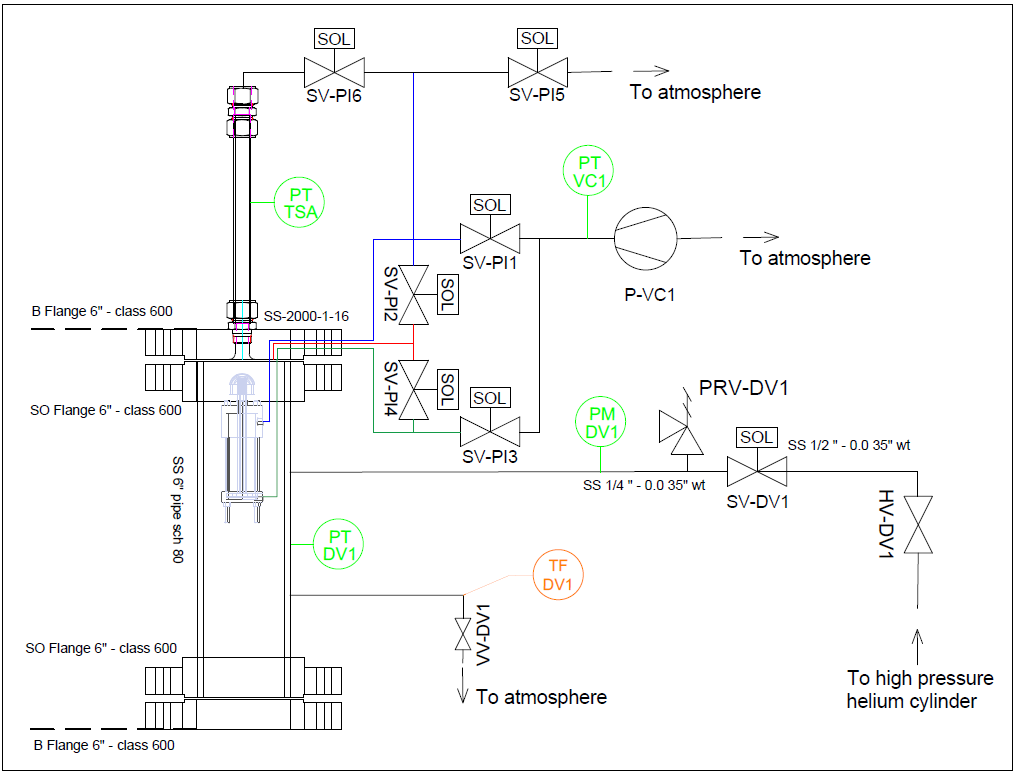
\includegraphics[width=0.55\textwidth]{experiment/photos/HENRI_valve_PID.PNG}
    \caption{Piping and instrumentation diagram (P\&ID) for piston valve operation.}
    \label{fig:sv pid}
    \vspace{16pt}
\end{figure}
%


The facility has pressure transducers distributed along its length, the major positions are highlighted in \Cref{fig:HENRI Facility}, and 1 thermocouple in the driver tank.
The pressure transducers are one of two main types: Omega PX459 or PCB 113B24.
All of the Omega pressure transducers are 0-\SI{10.3}{\mega\pascal} (0-1500 psia), except for two: a 0-\SI{24.1}{\mega\pascal} (0-3500 psia) transducer used on the driver tank, and a 0-\SI{0.103}{\mega\pascal} (0-15 psia) transducer used for the vacuum line.
The Omega pressure transducers output a current from 4-\SI{20}{\milli\amp}, which is converted to voltage using a \SI{250}{\ohm} shunt resistor.
The PCB transducers output a signal that is sent through a PCB Model 482C signal conditioner before being output to the voltage card.
The data acquisition system uses a National Instruments (NI) PXIe-1085 chassis with a NI PXIe-8135 controller, a NI PXIe-4303 voltage input card for reading the instrumentation, and a NI PXI-6515 digital output card for controlling the solenoid valves.
A LabVIEW program is used to record data from the chassis and to control the solenoid valves.
A piping and instrumentation diagram (P\&ID) for operating the piston valve can be seen in \Cref{fig:sv pid}.
There is a manifold of four (4) solenoid valves used to operate the piston. SV-PI2 and SV-PI4 open to fill the top and bottom chamber, respectively; and SV-PI1 and SV-PI3 open to vent the top and bottom chamber, respectively.
These solenoid valves are Parker Series 9 Miniature Calibrant Valve 009-0172-900.
This particular valve was selected for its small form factor, high pressure rating of \SI{8.6}{\mega\pascal} (1250 psi), and low helium leak rate of \SI{1e-7}{atm\ \centi\meter^3\per\second}.








% section for detailed experimental method (test matrix)
\subsection{Experimental Methodology} \label{ss:methodology}

% we tested the plugs and o-rings for durability / sealing with sustained seal tests and repeated seal tests outside of the henri facility (just using the flange and piston)
% we tested the valve / plugs / o-rings in henri tests

The overall methodology for testing the piston valve includes three main parts: comparing the piston valve's performance to the rupture disk; testing the piston valve's repeatability in HENRI helium insertions; and testing the piston valve for re-usability and sealing after large numbers of cycles. The piston valve is first tested in a HENRI injection and the results are compared to those of the rupture disk tests to ensure the piston valve is performing correctly and pressurizing the cartridge to the desired \SI{1.72}{\mega\pascal} (250 psi) in \SI{5}{\milli\second}. Secondly, the piston valve is tested repeatedly at one initial pressure to determine the repeatability of the valve, and at different initial pressures to determine how predictable the piston valve's behaviour is over a range of operating pressure. Thirdly, testing the re-usability of the piston valve was performed by cycling the piston valve to simulate the wear of long term use and comparing its sealing ability before and after the cycles. The LabVIEW code used for data acquisition was modified to automate the piston cycling process, so the cycle test could be performed overnight, then the piston valve is tested the next day to determine the seal degradation due to wear. A summary of the testing methodology is listed below.

\begin{itemize}
    \item Compare piston valve to rupture disk.
    \item Test repeatability at one pressure.
    \item Test piston valve operation at varying pressures.
    \item Test piston valve durability over time.
\end{itemize}